\documentclass[12pt,letterpaper]{article}
\usepackage{graphicx,textcomp}
\usepackage{natbib}
\usepackage{setspace}
\usepackage{fullpage}
\usepackage{color}
\usepackage[reqno]{amsmath}
\usepackage{amsthm}
\usepackage{fancyvrb}
\usepackage{amssymb,enumerate}
\usepackage[all]{xy}
\usepackage{endnotes}
\usepackage{lscape}
\newtheorem{com}{Comment}
\usepackage{float}
\usepackage{hyperref}
\newtheorem{lem} {Lemma}
\newtheorem{prop}{Proposition}
\newtheorem{thm}{Theorem}
\newtheorem{defn}{Definition}
\newtheorem{cor}{Corollary}
\newtheorem{obs}{Observation}
\usepackage[compact]{titlesec}
\usepackage{dcolumn}
\usepackage{tikz}
\usetikzlibrary{arrows}
\usepackage{multirow}
\usepackage{xcolor}
\newcolumntype{.}{D{.}{.}{-1}}
\newcolumntype{d}[1]{D{.}{.}{#1}}
\definecolor{light-gray}{gray}{0.65}
\usepackage{url}
\usepackage{listings}
\usepackage{color}

\definecolor{codegreen}{rgb}{0,0.6,0}
\definecolor{codegray}{rgb}{0.5,0.5,0.5}
\definecolor{codepurple}{rgb}{0.58,0,0.82}
\definecolor{backcolour}{rgb}{0.95,0.95,0.92}

\lstdefinestyle{mystyle}{
	backgroundcolor=\color{backcolour},   
	commentstyle=\color{codegreen},
	keywordstyle=\color{magenta},
	numberstyle=\tiny\color{codegray},
	stringstyle=\color{codepurple},
	basicstyle=\footnotesize,
	breakatwhitespace=false,         
	breaklines=true,                 
	captionpos=b,                    
	keepspaces=true,                 
	numbers=left,                    
	numbersep=5pt,                  
	showspaces=false,                
	showstringspaces=false,
	showtabs=false,                  
	tabsize=2
}
\lstset{style=mystyle}
\newcommand{\Sref}[1]{Section~\ref{#1}}
\newtheorem{hyp}{Hypothesis}

\title{Problem Set 3}
\date{Zexi Wang}
\author{Applied Stats/Quant Methods 1}


\begin{document}
	\maketitle
	\section*{Instructions}
	\begin{itemize}
		\item Please show your work! You may lose points by simply writing in the answer. If the problem requires you to execute commands in \texttt{R}, please include the code you used to get your answers. Please also include the \texttt{.R} file that contains your code. If you are not sure if work needs to be shown for a particular problem, please ask.
	\item Your homework should be submitted electronically on GitHub.
	\item This problem set is due before 23:59 on Sunday November 11, 2024. No late assignments will be accepted.

	\end{itemize}

		\vspace{.25cm}
	
\noindent In this problem set, you will run several regressions and create an add variable plot (see the lecture slides) in \texttt{R} using the \texttt{incumbents\_subset.csv} dataset. Include all of your code.

	\vspace{.5cm}
\section*{Question 1}
\vspace{.25cm}
\noindent We are interested in knowing how the difference in campaign spending between incumbent and challenger affects the incumbent's vote share. 
	\begin{enumerate}
		\item Run a regression where the outcome variable is \texttt{voteshare} and the explanatory variable is \texttt{difflog}.
		\lstinputlisting[language=R, firstline=33, lastline=39]{PS3_ZexiWang.R}
		\begin{verbatim}
			===============================================
			Dependent variable:    
			---------------------------
			voteshare         
			-----------------------------------------------
			difflog                  0.042*** (0.001)      
			Constant                 0.579*** (0.002)      
			-----------------------------------------------
			Observations                   3,193           
			R2                             0.367           
			Adjusted R2                    0.367           
			Residual Std. Error      0.079 (df = 3191)     
			F Statistic         1,852.791*** (df = 1; 3191)
			===============================================
			Note:               *p<0.1; **p<0.05; ***p<0.01
		\end{verbatim} 

		\item Make a scatterplot of the two variables and add the regression line. 	
		\lstinputlisting[language=R, firstline=41, lastline=50]{PS3_ZexiWang.R} 
		\begin{figure}[H]
			\centering
			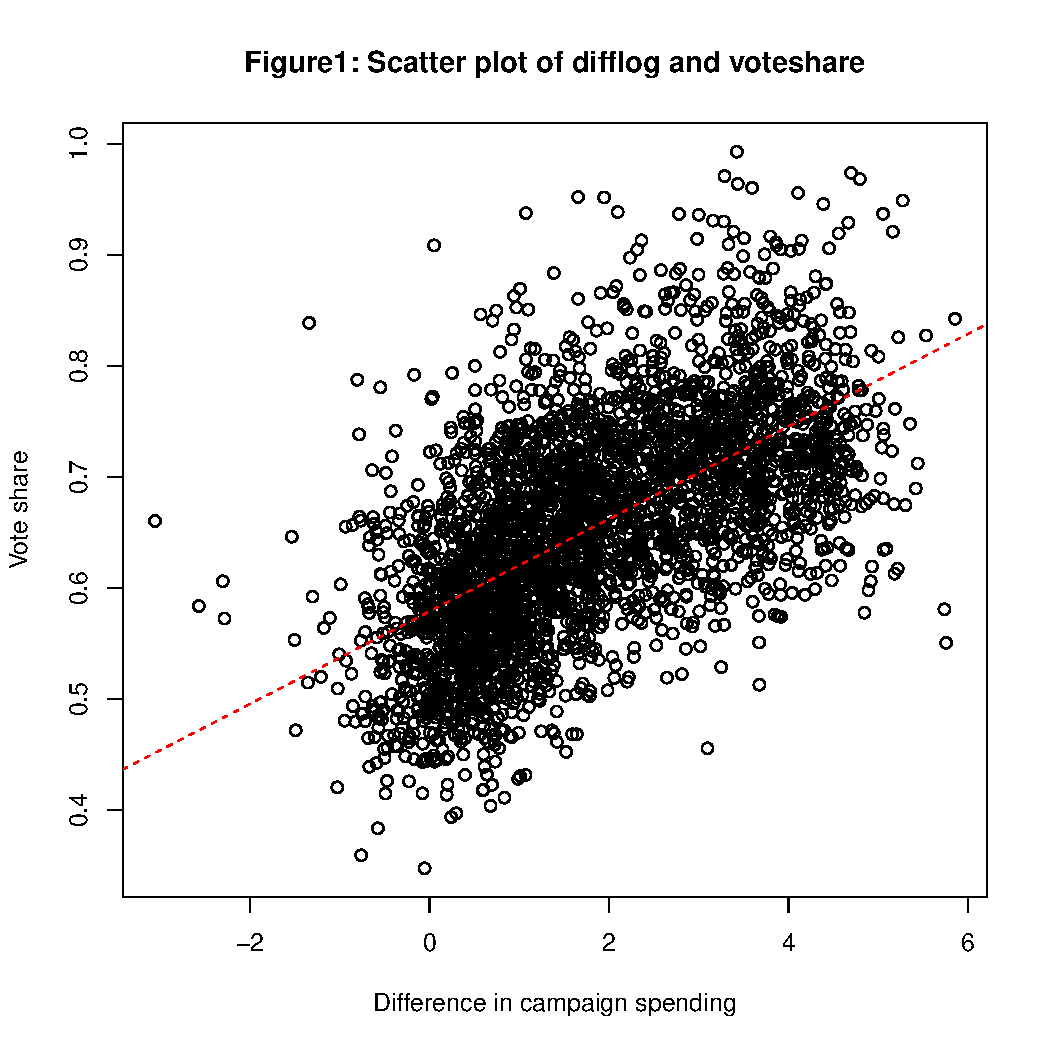
\includegraphics[width=.5\textwidth]{Q1_2_scatterplot.pdf}
		\end{figure}

		\item Save the residuals of the model in a separate object.	
		\lstinputlisting[language=R, firstline=51, lastline=54]{PS3_ZexiWang.R} 
		
		\item Write the prediction equation.
		\begin{align*}
			voteshare = 0.579 + 0.042 \times \text{difflog}
		\end{align*}
	\end{enumerate}
	

\section*{Question 2}
\noindent We are interested in knowing how the difference between incumbent and challenger's spending and the vote share of the presidential candidate of the incumbent's party are related.	\vspace{.25cm}
	\begin{enumerate}
		\item Run a regression where the outcome variable is \texttt{presvote} and the explanatory variable is \texttt{difflog}.
		\lstinputlisting[language=R, firstline=55, lastline=60]{PS3_ZexiWang.R} 
		\begin{verbatim}
			===============================================
			Dependent variable:    
			---------------------------
			presvote          
			-----------------------------------------------
			difflog                  0.024*** (0.001)      
			Constant                 0.508*** (0.003)      
			-----------------------------------------------
			Observations                   3,193           
			R2                             0.088           
			Adjusted R2                    0.088           
			Residual Std. Error      0.110 (df = 3191)     
			F Statistic          307.715*** (df = 1; 3191) 
			===============================================
			Note:               *p<0.1; **p<0.05; ***p<0.01
		\end{verbatim} 
		
		\item Make a scatterplot of the two variables and add the regression line.
		\lstinputlisting[language=R, firstline=61, lastline=69]{PS3_ZexiWang.R} 
		\begin{figure}[H]
			\centering
			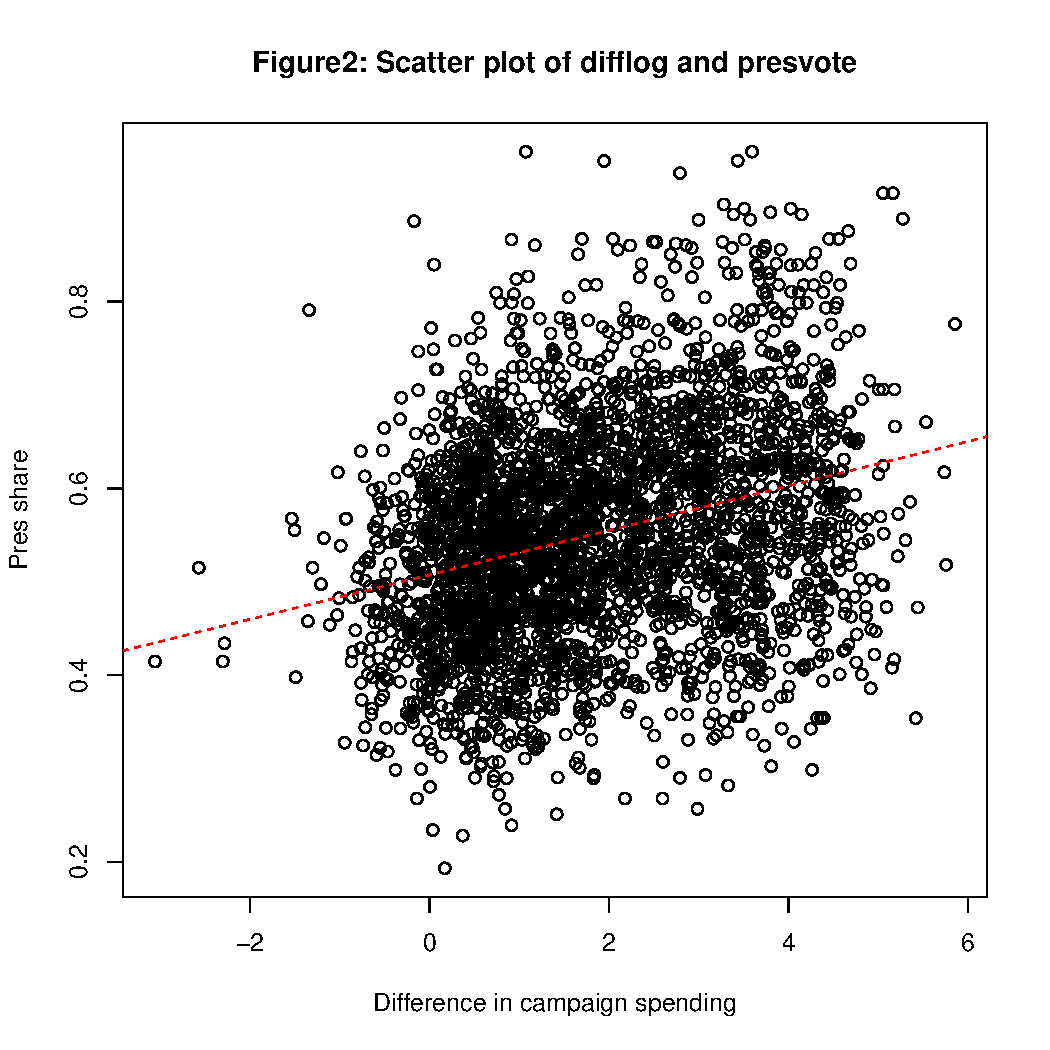
\includegraphics[width=.55\textwidth]{Q2_2_scatterplot.pdf}
		\end{figure}
		
		\item Save the residuals of the model in a separate object.	
		\lstinputlisting[language=R, firstline=71, lastline=73]{PS3_ZexiWang.R} 
		
		\item Write the prediction equation.
		\begin{align*}
			presvote &= 0.508 + 0.024 \times \text{difflog}
		\end{align*}
	\end{enumerate}
\newpage
		
\section*{Question 3}

\noindent We are interested in knowing how the vote share of the presidential candidate of the incumbent's party is associated with the incumbent's electoral success.
	\vspace{.25cm}
	\begin{enumerate}
		\item Run a regression where the outcome variable is \texttt{voteshare} and the explanatory variable is \texttt{presvote}.
		\lstinputlisting[language=R, firstline=75, lastline=80]{PS3_ZexiWang.R}
		\begin{verbatim}
			===============================================
			Dependent variable:    
			---------------------------
			voteshare         
			-----------------------------------------------
			presvote                 0.388*** (0.013)      
			Constant                 0.441*** (0.008)      
			-----------------------------------------------
			Observations                   3,193           
			R2                             0.206           
			Adjusted R2                    0.206           
			Residual Std. Error      0.088 (df = 3191)     
			F Statistic          826.950*** (df = 1; 3191) 
			===============================================
			Note:               *p<0.1; **p<0.05; ***p<0.01
		\end{verbatim}  

		\item Make a scatterplot of the two variables and add the regression line. 
		\lstinputlisting[language=R, firstline=81, lastline=90]{PS3_ZexiWang.R} 
		\begin{figure}[H]
			\centering
			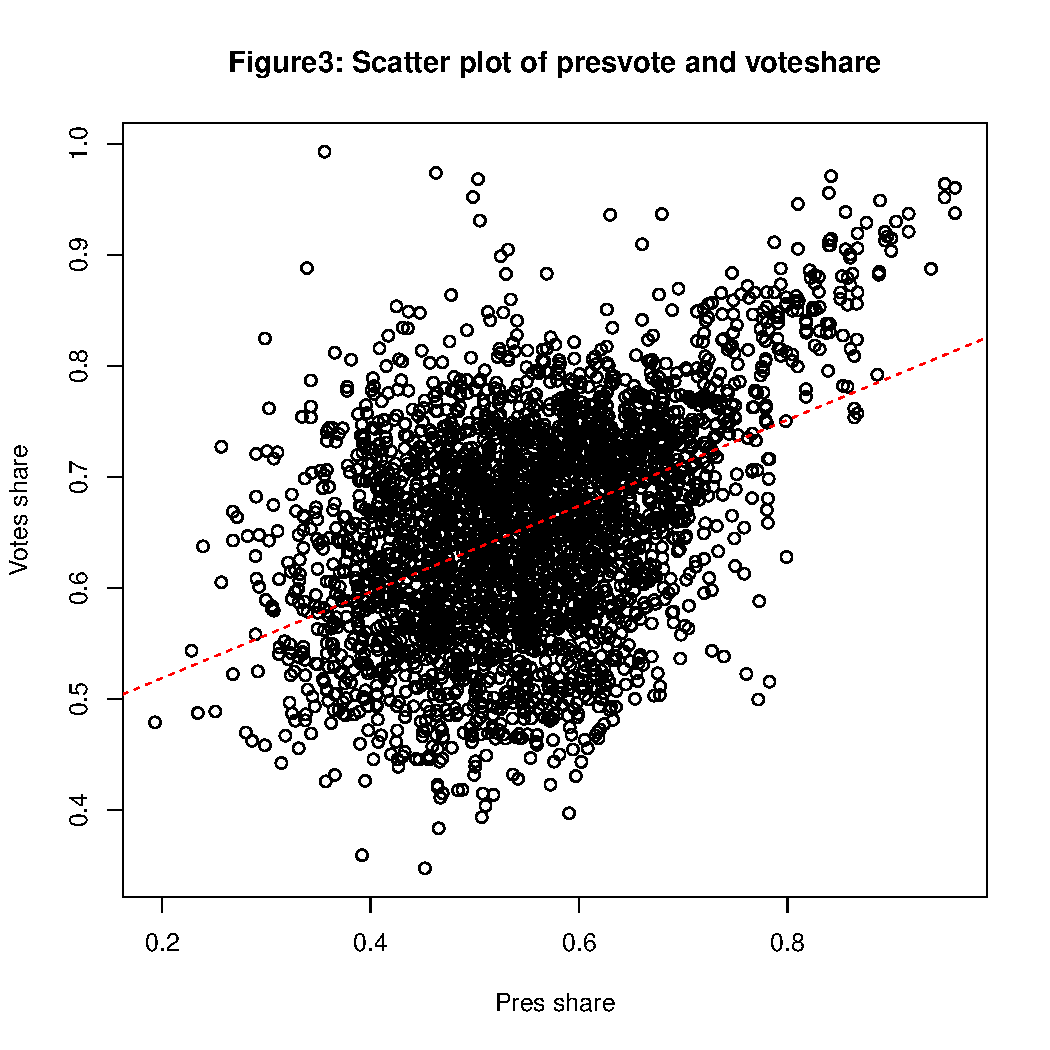
\includegraphics[width=.55\textwidth]{Q3_2_scatterplot.pdf}
		\end{figure}
		
		\item Write the prediction equation.
		\begin{equation*}
			voteshare = 0.441 + 0.388 \times presvote
		\end{equation*}
		
	\end{enumerate}
	

\newpage	
\section*{Question 4}
\noindent The residuals from part (a) tell us how much of the variation in \texttt{voteshare} is $not$ explained by the difference in spending between incumbent and challenger. The residuals in part (b) tell us how much of the variation in \texttt{presvote} is $not$ explained by the difference in spending between incumbent and challenger in the district.
	\begin{enumerate}
		\item Run a regression where the outcome variable is the residuals from Question 1 and the explanatory variable is the residuals from Question 2.
		\lstinputlisting[language=R, firstline=94, lastline=99]{PS3_ZexiWang.R}
		\begin{verbatim}
		 	================================================
		 	Dependent variable:    
		 	---------------------------
		 	model_vote_dif_resid    
		 	------------------------------------------------
		 	model_pres_dif_resid      0.257*** (0.012)      
		 	Constant                   -0.000 (0.001)       
		 	------------------------------------------------
		 	Observations                    3,193           
		 	R2                              0.130           
		 	Adjusted R2                     0.130           
		 	Residual Std. Error       0.073 (df = 3191)     
		 	F Statistic           476.975*** (df = 1; 3191) 
		 	================================================
		 	Note:                *p<0.1; **p<0.05; ***p<0.01
		 \end{verbatim}  
		
		\item Make a scatterplot of the two residuals and add the regression line. 	
		\lstinputlisting[language=R, firstline=100, lastline=109]{PS3_ZexiWang.R} 
     	\begin{figure}[H]
			\centering
			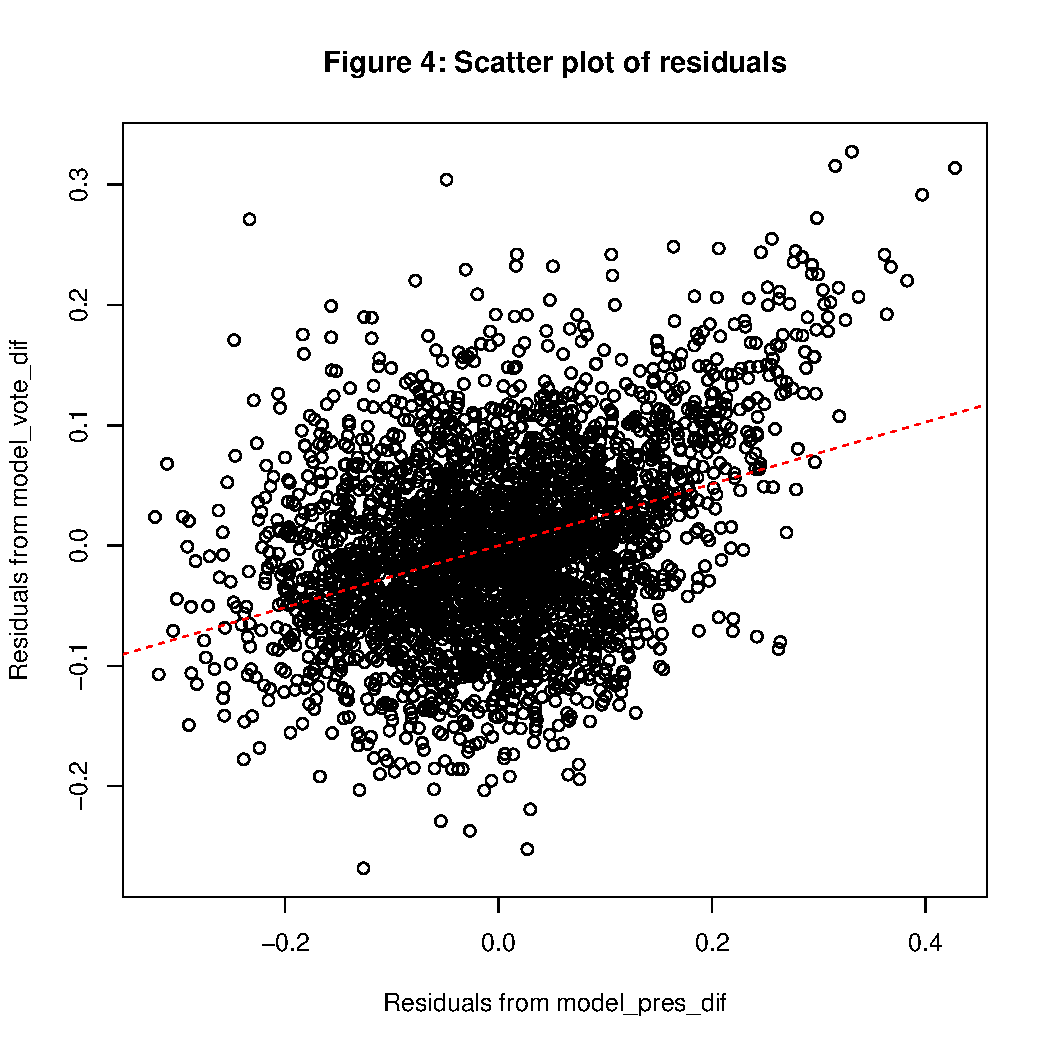
\includegraphics[width=.55\textwidth]{Q4_2_scatterplot.pdf}
		\end{figure}
		
		\item Write the prediction equation.
		\begin{equation*}
			\tt{model\_pres\_dif\_residuals} = 0 + 0.257 \times \tt{model\_vote\_dif\_residuals}
		\end{equation*}
	\end{enumerate}	
	
\newpage
\section*{Question 5}
\noindent What if the incumbent's vote share is affected by both the president's popularity and the difference in spending between incumbent and challenger? 
	\begin{enumerate}
		\item Run a regression where the outcome variable is the incumbent's \texttt{voteshare} and the explanatory variables are \texttt{difflog} and \texttt{presvote}.	
		\lstinputlisting[language=R, firstline=110, lastline=115]{PS3_ZexiWang.R}
		\begin{verbatim}
			===============================================
			Dependent variable:    
			---------------------------
			voteshare         
			-----------------------------------------------
			difflog                  0.036*** (0.001)      
			presvote                 0.257*** (0.012)      
			Constant                 0.449*** (0.006)      
			-----------------------------------------------
			Observations                   3,193           
			R2                             0.450           
			Adjusted R2                    0.449           
			Residual Std. Error      0.073 (df = 3190)     
			F Statistic         1,302.947*** (df = 2; 3190)
			===============================================
			Note:               *p<0.1; **p<0.05; ***p<0.01
		\end{verbatim} 
		
		\item Write the prediction equation.
		\begin{equation*}
			voteshare = 0.449 + 0.036 \times difflog + 0.257 \times presvote
		\end{equation*}
		
		\item What is it in this output that is identical to the output in Question 4? Why do you think this is the case?
		\begin{verbatim}
			This phenomenon occurs because the two coefficients actually describe 
			the same relationship - the residual association between presvote 
			and voteshare after controlling for difflog.
		\end{verbatim} 

		
		
	\end{enumerate}




\end{document}
